\DiaryEntry{Groups, III}{2016-03-04}{Algebra}

\subsection{Cyclic Groups}\label{cyclic-groups}

Cyclic groups are denoted as \(C_n\) and are defined by
\(G =\langle a \rangle\) where \(a\) is the \textbf{generator} of G.

Simplest examples for cyclic groups are the integers with modulo-n
addition; i.e. \(\mathbb{Z}_n\).

The following Figure shows Cayley diagrams for \(n=3\) and \(n=5\).

\begin{figure}[H]
\centering
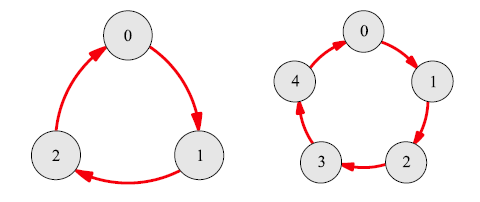
\includegraphics{images/groups_03_1.png}
\caption{Page1}
\end{figure}

The left diagram shows the group elements \(1,2,3\) and the effect the
operation \((x + 1) \mod 3\) has on each group element as the red lines
(with arrows). Note that selecting another operation (e.g.
\((x + 2) \mod 3\)) would make the lines look different.

The right figure shows the same for the group elements \(1,2,3,4,5\) and
operation \((x + 1) \mod 5\).

Another example for a cyclic group are the (complex) roots of unity
under (complex) multiplication; i.e.

\[
x_k = \exp \frac{2\pi i}{N} k, \quad k=0,\ldots,N-1
\]

We have that \(x_k x_k\) is an element of the group and the identity
element is \(1\). Therefore, the elements \(x_k\) for a group.
Furthermore, the group is cyclic with generator being \(x_1\).

\subsection{Permutation Groups}\label{permutation-groups}

The permutations of a set form a group; if the set is the numbers from
1\ldots{}n, the group is the symmetric group \(S_n\). The group has
\(n!\) elements and the binary operation is the composition of
permutations. Note that permutations are not commutative in general.

A permutation group has several subgroups; as an example consider the
subgroup of \(G_5\) consisting of the identitiy element and the
following elements

\[
\sigma =
\begin{pmatrix}
1 & 2 & 3 & 4 & 5 \\
1 & 2 & 3 & 5 & 4
\end{pmatrix}
,\quad \tau = 
\begin{pmatrix}
1 & 2 & 3 & 4 & 5 \\
3 & 2 & 1 & 4 & 5
\end{pmatrix}
, \quad \mu = 
\begin{pmatrix}
1 & 2 & 3 & 4 & 5 \\
3 & 2 & 1 & 5 & 4
\end{pmatrix}
\]

The following table shows how to multiply elements in this subgroup:

\[
\begin{array}{c|cccc}
\star   & e     & \sigma & \tau   & \mu    \\
\hline
e     & e     & \sigma & \tau   & \mu    \\
\sigma & \sigma & e     & \mu    & \tau   \\
\tau   & \tau   & \mu    & e     & \sigma \\
\mu    & \mu    & \tau   & \sigma & e
\end{array}
\]

\subsubsection{Cycle Notation}\label{cycle-notation}

This is a shorthand notation for writing permutations. The cycle
notation lists all cycles of a permutation. For example, the permutation
\(\sigma\) is in cycle notation \((4,5)\), for \(\tau\) it is \((1,3)\),
and for \(\mu\) it is \((1,3)(4,5)\). Elements which are not part of a
cycle are not listed; that is the elements \(1,2,3\) are left in place
by the permutation \(\sigma\). Besides, note that permutations can also
contain more than one cycle.

As another example consider the permutation

\[
\begin{pmatrix}
1 & 2 & 3 & 4 & 5 & 6 \\
2 & 4 & 1 & 3 & 6 & 5
\end{pmatrix}
\]

which has cycle notation \((1,2,4,3)(5,6)\). Note that the order of the
elements in the cycle is important; i.e.~cycles \((1,2,4,3)\) and
\((1,2,3,4)\) denote different cycles.

\subsubsection{More on Cylces}\label{more-on-cylces}

Cycles can be multiplied; for example if we have \(\sigma=(1,3,5,2)\)
and \(\tau = (2,5,6)\), then the product \(\sigma \tau\) can be obtained
by considering the effect of \(\sigma \tau\) on every integer: We have
\(\sigma (\tau (1)) = \sigma(1) = 3\),
\(\sigma (\tau (2)) = \sigma(5) = 2\),
\(\sigma (\tau (3)) = \sigma(3) = 5\),
\(\sigma (\tau (4)) = \sigma(4) = 4\),
\(\sigma (\tau (5)) = \sigma(6) = 6\),
\(\sigma (\tau (6)) = \sigma(2) = 1\). Converting this into cycle
notation, we obtain for the product \(\sigma \tau = (1,3,5,6)\)

Two cycles are disjoint if they contain different elements. If
\(\sigma\) and \(\tau\) are disjoint cycles, then
\(\sigma \tau = \tau \sigma\).

Proof: For elements in neither cycle, both \(\sigma\) and \(\tau\) leave
these elements untouched, therefore order of permutations is not
important. If an element is contained in one cycle it is not contained
in the other cycle (by definition of disjointness) and therefore not
touched by this permutation.

Assume that \(a\) is contained in \(\sigma\), but not in \(\tau\).
Therefore \(\tau(a) = a\) and \(\sigma(\tau(a)) = \sigma(a)\) and
\(\tau(\sigma(a)) = \sigma(a)\). The argument stays the same when \(a\)
is contained in \(\tau\) instead.

Every permutation in \(S_n\) can be expressed as product of disjoint
cycles.

A transposition is a cylce of length 2; i.e.~an element exchange. Any
permutation of finite elements with at least 2 elements can be written
as product of transpositions (not necessarily disjoint).

As an example, consider the product of
\(\sigma_1 \sigma_2 = (2,4)(2,6)\). We need only to consider what
happens to the element \(2,4,6\) as all other elements are outside the
cycle(s). Therefore, we have \(\sigma_1(\sigma_2(2)) = 6\),
\(\sigma_1(\sigma_2(4)) = 2\), \(\sigma_1(\sigma_2(6)) = 4\). Combining
this into a cycle yields \((2,6,4)\). From this we deduce the general
rule that

\[
(a,b)(a,c) = (a,c,b), \quad \mbox{and} \quad (a,b)(a,c)(a,d) = (a,d,c,b)
\]

There is no unique way of writing permutations as product of
transpositions; however, the number of transpositions to express a
permutation is a constant. We define a permutation to be \textbf{even},
if it can be expressed as an even number of transpositions and
\textbf{odd} if it can be expressed as an odd number of transpositions.

\subsection{Alternating Groups}\label{alternating-groups}

One of the most important subgroups of \(S_n\) is the set of all even
permutations, \(A_n\), the alternating group on n elements. \(A_n\) is a
subgroup of \(S_n\).
